% MA211 - Lecture 14
\documentclass[pdftex, xcolor=pdftex, dvipsnames,handout]{beamer}

\usetheme{MA211}
\usepackage{thumbpdf}
\usepackage{wasysym}
%\usepackage{ucs}
\usepackage[utf8]{inputenc}
\usepackage{pgf,pgfarrows,pgfnodes,pgfautomata,pgfheaps,pgfshade}
\usepackage{verbatim}

\usepackage{eurosym}
\usepackage{euler}

\usepackage{calc}               % Simple computations with LaTeX variables
%\usepackage[hang]{caption2}     % Improved captions

\usepackage{graphicx}           % Standard graphics package

\usepackage{amsmath, amsthm, amssymb}


\newcommand{\fquad}{\mbox{\qquad}}
\newcommand{\bull}{$\bullet$ }

\newcommand {\I} {\mathcal I}
\newcommand {\calI} {\mathcal I}
\def\disint{\displaystyle\int}

\DeclareMathOperator{\D}{d}
\newcommand{\dydx}{\frac{\D y}{\D x}}

%\definecolor{gray}{rgb}{0.69, 0.69, 0.69} \newcommand{\gray}[1]{\textcolor{gray}{#1}}
\definecolor{dogreen}{rgb}{0.33, 0.42, 0.18} \newcommand{\dogreen}[1]{\textcolor{dogreen}{#1}}
\definecolor{maroon}{rgb}{.5,0.2,0.2}\newcommand{\maroon}[1]{\textcolor{maroon}{#1}}
\definecolor{greena}{rgb}{.1,0.581,0.1}\newcommand{\greena}[1]{\textcolor{greena}{#1}}

\definecolor{blue4}{rgb}{0,0,.545}
\newcommand{\Blue}[1]{\textcolor{blue}{#1}}
\newcommand{\Red}[1]{\textcolor{red}{#1}}
\definecolor{pink}{rgb}{1.,0.75,0.8}
\definecolor{darkred}{rgb}{0.5,0.0,0.0}
\definecolor{darkgreen}{rgb}{0,0.3,0.3}
\definecolor{purple}{rgb}{0,0.3,0.3}
\definecolor{darkblue}{rgb}{0.0, 0.0, .5}
\definecolor{dpurple}{rgb}{.3,.0,.3}
\newcommand{\Green}[1]{\textcolor{darkgreen}{#1}}
\newcommand{\DRed}[1]{\textcolor{darkred}{#1}}
\newcommand{\DBlue}[1]{\textcolor{darkblue}{#1}}
\newcommand{\Purple}[1]{\textcolor{dpurple}{#1}}
\newcommand{\Emph}[1]{\textcolor{darkred}{\textbf{\it #1}}}
\newcommand{\remph}[1]{\textcolor{darkred}{\textbf{\emph{#1}}}}
\newcommand{\bemph}[1]{\textcolor{darkblue}{\textbf{\emph{#1}}}}
\newcommand{\gemph}[1]{\textcolor{darkgreen}{\textbf{\emph{#1}}}}
\newcommand{\Bf}[1]{\textcolor{darkblue}{\textbf{#1}}}
\newcommand{\Gf}[1]{\textcolor{darkgreen}{\textbf{#1}}}
\newcommand{\Rf}[1]{\textcolor{red}{\textbf{#1}}}
\newcommand{\Rmf}[1]{\textcolor{red}{\mathbf{#1}}}

\newcommand{\Conj}[1]{\overline{#1}}

\newcommand{\code}[1]{\textcolor{darkblue}{\texttt{\textbf{#1}}}}
\newcommand{\icode}[1]{{\blue\texttt{\textbf{\emph{#1}}}}}
\newcommand{\gcode}[1]{{\Green{\texttt{\textbf{\emph{#1}}}}}}
\newcommand{\out}[1]{\texttt{\emph{\textbf{\Green{#1}}}}}





\newenvironment{vminipage}%
{\begin{Sbox}\begin{minipage}\begin{small}\begin{verbatim}}%
{\end{verbatim}\end{small}\end{minipage}\end{Sbox}\fbox{\TheSbox}}

\newenvironment{nminipage}%
{\begin{Sbox}\begin{minipage}}%
{\end{minipage}\end{Sbox}\fbox{\TheSbox}}


\let\Arg\relax\DeclareMathOperator{\Arg}{\mathtt{Arg}}
\let\Arg\relax\DeclareMathOperator{\e}{\mathtt{e}}

\newcommand {\AND} {\wedge}
\newcommand {\OR} {\vee}
\newcommand {\NOT} {\neg}
\newcommand {\IMPLIES} {\rightarrow}
%\newcommand {\IFF} {\leftrightarrow}
\renewcommand {\iff} {\Leftrightarrow}
\newcommand {\NAND} {\uparrow}
\newcommand {\NOR} {\downarrow}
\newcommand {\XOR} {\otimes}

\newenvironment{citemize}% Colour items
{\begin{description}}%
{\end{description}}

\newcommand {\maroonitem}{\item[\maroon{$\bullet$}]}

\newcommand {\gitem} {\item {\includegraphics[width=.4cm,angle=-10]{img/green-bullet-on-white.ps}}}
\newcommand {\ritem} {\item {\includegraphics[width=.4cm,angle=-10]{img/red-bullet-on-white.ps}}}
\newcommand {\yitem} {\item {\includegraphics[width=.4cm,angle=-10]{img/yellow-bullet-on-white.ps}}}
\newcommand {\bitem} {\item {\includegraphics[width=.4cm,angle=-10]{img/blue-bullet-on-white.ps}}}

\newcommand {\greenitem} {\item {\includegraphics[width=.4cm,angle=-10]{img/green-bullet-on-white.ps}}}
\newcommand {\reditem} {\item {\includegraphics[width=.4cm,angle=-10]{img/red-bullet-on-white.ps}}}
\newcommand {\yellowitem} {\item {\includegraphics[width=.4cm,angle=-10]{img/yellow-bullet-on-white.ps}}}
\newcommand {\blueitem} {\item {\includegraphics[width=.4cm,angle=-10]{img/blue-bullet-on-white.ps}}}

\newcommand {\eq}[1]%
  {$\DBlue{#1}$}
\newcommand {\eqd}[1]%
  {$\displaystyle\DBlue{#1}$}
%\newcommand{\eq}[1]{\boldmath \DBlue{$#1$}}


\newcommand {\csf}{\centerslidesfalse}
\newcommand {\cst}{\centerslidestrue}

\newcommand {\vecii}[2] {   \big(\begin{smallmatrix} #1 \\ #2 \end{smallmatrix}\big)}
\newcommand{\atwo}[2]{\left(\!\!\begin{array}{c} #1 \\ #2 \end{array}\!\!\right)}


\newcommand{\C}{\mathbb{C}}
\newcommand{\Q}{\mathbb{Q}}
\newcommand{\R}{\mathbb{R}}
\newcommand{\N}{\mathbb{N}}
\newcommand{\Z}{\protect\mathbb{Z}}  % protect for index.
\newcommand {\Rs}{ \mathbb{R}}
\newcommand {\Cs}{ \mathbb{C}}
\newcommand {\Rnn}{ \mathbb{R}^{n \times n}}
\newcommand {\Rn}{ \mathbb{R}^{n}}


\newcommand{\mblock}{%
\setbeamercolor*{block title}{bg=maroon,fg=white}
\setbeamercolor*{block body}{bg=white,fg=maroon}
}%

\newcommand{\bblock}{%
\setbeamercolor*{block title}{bg=Steel,fg=white}
\setbeamercolor*{block body}{bg=Mylightgray,fg=Steel}
}%

\newcommand{\gblock}{%
\setbeamercolor*{block title}{bg=Green,fg=white}
\setbeamercolor*{block body}{bg=Mylightgray,fg=darkgreen}
}%


\newcommand{\rblock}{%
\setbeamercolor*{block title}{bg=Red,fg=white}
\setbeamercolor*{block body}{bg=white,fg=Black}
}%


\newcommand{\TakeNotes}{
\includegraphics[width=2cm]{TakeNote}}

\def\eps{\varepsilon}
\newcommand {\del}[2]{ {\frac{\partial #1}{\partial #2}}}
\newcommand {\x}[1]{x^{[#1]}}
\newcommand {\delx}{ {\frac{\partial}{\partial x}}}
\newcommand {\delt}{ {\frac{\partial}{\partial t}}}
\newcommand {\dely}{ {\frac{\partial}{\partial y}}}
\newcommand {\ith}{{(i)}}
\renewcommand {\vec}[1]{ {\boldsymbol{#1}}}
\newcommand {\Oh} {\mathcal O}
\newcommand {\Err} {\mathcal E}
%\newcommand {\th} {\mathrm{th}}
\DeclareMathOperator{\fl}{fl}
\DeclareMathOperator{\sign}{sign}
\DeclareMathOperator{\Cond}{Cond} 
\DeclareMathOperator{\cond}{cond}
\DeclareMathOperator{\diag}{diag} 
\DeclareMathOperator{\sym}{sym} 
\DeclareMathOperator{\Trace}{Trace}
%\DeclareMathOperator{\D}{d}
\DeclareMathOperator{\E}{e}

\newcommand {\Rsym}{{ \mathbb{R}^{n \times n}_\mathrm{sym}}}

\newcommand {\st} {\mathrm{st}}
\newcommand {\nd} {\mathrm{nd}}


\parskip .25cm


\theoremstyle{definition}
\newtheorem{exercise}{Exercise}[section]
\newtheorem{method}{Method}[section]

\newcommand{\Header}[1]{\begin{center}{\Large \Bf{#1}}\end{center}}

\subtitle{MA211}
\title{Lecture 14: Nonhomogeneous DEs (continued)}

\author{Dr Niall Madden}

\date{\Large Wed $22^\mathrm{nd}$ October  2008}


\begin{document}

\setcounter{framenumber}{-1}
\frame{

\begin{block}{}
\begin{center}
{\large \insertsubtitle}

\vspace{.1cm}

\begin{large}
\textbf{\inserttitle}
\end{large}

\vspace{.15cm}

% {\footnotesize \insertauthor}

\vspace{.3cm}

{ {\insertdate}}
\end{center}
\end{block}


\vspace{-0.25cm}
\begin{center}
%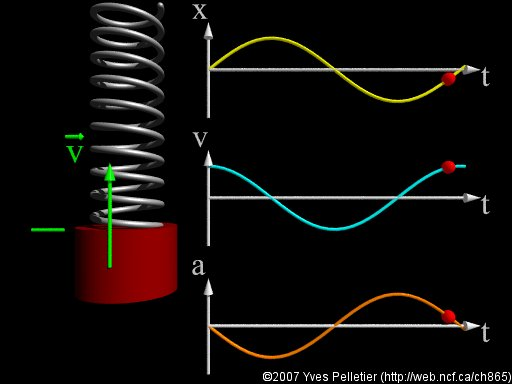
\includegraphics[height=4cm]{images/SHM.jpg}

\end{center}
}




\frame{
  \frametitle{Today...}

 \tableofcontents


For further details and examples, look at the section on
\Emph{Nonhomogeneous Linear Equations}, Section 17.2 of Stewart
\Emph{Calculus: early transcendentals}.

}

\section{Non-homogeneous Problems}

\frame{
On Monday we began the section of the course that deals with solving
problems of the form

\begin{block}{Non-Homogeneous}
\[ ay'' + by' + cy =  \Rf{f(x)}. \]
\end{block}
where 
\begin{enumerate}
\item \eq{f} is a polynomial. (\alert{done in Lecture 13})
\item \eq{f=Ke^{Tx}} for some numbers  \eq{K} and \eq{T} (started
  \alert{in Lecture 13}).

\item \eq{f} is a trig function, such as \eq{\sin} and \eq{\cos}

\item Some combination of the above.
\end{enumerate}

The technique we introduced is  sometimes called the \Emph{method of
  undetermined  coefficients}.

}


\section{$f(x)=Ke^{Tx}$}


\frame{
If the right-hand side of the DE is an exponential function:
\rblock
\begin{block}{\eq{f = Ke^{Tx}}}
When solving the Non-homogeneous DE\\
\hspace{2cm} \eq{  ay'' + by' + cy = \Rf{f(x)}}. \qquad 
where \eq{f = Ke^{Tx}}:\\
\begin{enumerate}%[<+->]
\item Solve the homogeneous DE \eq{ah'' + bh' + ch = \Rf{0}}. 


\item Check if term \eq{e^Tx} appears in \eq{h}, and choose \eq{u} to
  be one of 
 \eq{Me^{Tx}}, \eqd{Mxe^{Tx}} or \eqd{Mx^2 e^{Tx}}
 accordingly. Specifically:
\begin{itemize} 
\item If \eq{T} is \Emph{not} a solution to the auxiliary equation,
  set \eq{u= M e^{Tx}}.
\item If  the auxiliary equation has \Emph{two} distinct solutions,
  and one of them is \eq{T},  set \eq{u= Mx e^{Tx}}.
\item If  the auxiliary equation has just \Emph{one} solution,
  and that is \eq{T}, set \eq{u= Mx^2 e^{Tx}}.
\end{itemize}

\item Substitute \eq{u} into the DE, divide by \eq{e^{Tx}} and solve
  for \eq{M}.
\item The general solution is then \eq{y(x)= h(x) + u(x)}.
\end{enumerate} 
\end{block}
}


\frame{

In the  two example that we did at the end on Monday's lecture, \eq{f}
did not appear in the solution to the complementary homogeneous
equation.

Now we'll do two examples where it does.


}


\frame{
\begin{example}
Solve the following DE
\[
2 y''  +  y' - y = 3e^{x/2}.
\]
\end{example}

\vspace{4.5cm}
}

\frame{
\begin{example}
Solve the following DE
\[
 y''  +  2y' + y = 4e^{-x}.
\]
\end{example}

\vspace{4.5cm}
}



\frame{

\begin{exercise}[Q14.1]
Find general solutions to the following non-homogeneous differential equations:
\begin{enumerate}
\item $y'' + y' - 2y =e^{-x}$.
\item $y'' + y' - 2y = 3e^x$.
\item $y'' + 5y' + 6y = 4e^{-2x}$.
\item  $-3y'' + 3y' -y = \frac{1}{2}e^{-x/2}$.
\end{enumerate}

\end{exercise} 

\begin{exercise}[Q14.2]
Suppose the solution to \eqd{ah'' + bh' + ch = 0}, where
  $D=b^2-4ac >0$ so  $h$ is of the form \eq{h=Ae^{R_1x} + Be^{R_2x}}.

Show that, if \eq{u} is a \emph{particular} solution to 
\eqd{au'' + bu' + cu = Ke^{R_1x}},  then 
 \eq{u=\frac{K}{\sqrt{D}} x e^{R_1x}}.

\end{exercise} 
}

\section{$f$ is a trigonometric function}

\frame{
%If the right-hand side of the DE is a trig function (\eq{\cos} or
%\eq{\sin}):
\rblock
\begin{block}{$f$ is $\sin(Tx)$ or $\cos(Tx)$}
When solving the Non-homogeneous DE\\
\hspace{2cm} \eq{  ay'' + by' + cy = \Rf{f(x)}}.\\
where \eq{f} is \eq{\sin(Tx)} or \eq{\cos(Tx)}:\\
\begin{enumerate}[<+->]
\item Solve the homogeneous DE \eq{ah'' + bh' + ch = \Rf{0}}.
\begin{itemize}
\item If \eq{f} does \Emph{not} appear as part of \eq{h}, set
 \eq{u = z_1 \sin(Tx) + z_2\cos(Tx)}, where \eq{z_1} and
  \eq{z_2} are some numbers.
\item If \eq{f}  \Emph{does} appear as part of \eq{h}, set
 \eq{u = z_1 x\sin(Tx) + z_2 x\cos(Tx)}.
\end{itemize}
\item Substitute \eq{u} into the DE. Get 2 equations: one for
  \eq{\sin}  and one for \eq{cos}.
\item Solve the 2 equations for \eq{z_1} and \eq{z_2}.

\item The general solution is then \eq{y(x)= h(x) + z_1 \sin(x) + z_2 \cos(x)}.
\end{enumerate} 
\end{block}
}



\frame{
\begin{example}
Find the general solution to the non-homogeneous problem:
\[
4 y''  + 12 y' + 9y = \sin(\frac{x}{2}).
\]

\end{example}

\vspace{4.5cm}
}



\frame{
\begin{example}
Find the general solution to the non-homogeneous problem:
\[
y''  + 4 y = \cos(2x).
\]

\end{example}

\vspace{4.5cm}
}

\frame{
\begin{exercise}[Q14.3]
 Find general solutions to the following differential equations:
\begin{enumerate}
\item $y'' - y =\cos(x)$.
\item $y'' + y' - 2y =5\sin(-2x)$.
\end{enumerate}
\end{exercise}

See also Exer 14.4 on Problem Set 3.

}


\section{$f$ is the sum of two functions}
\frame{
Now we can solve each of the following problems:\\
\hspace{2cm} \eq{  ay'' + by' + cy = \alert{P(x)}}.\\ 
\hspace{2cm} \eqd{ ay'' + by' + cy =  \alert{e^{Tx}}}.\\ 
\hspace{2cm} \eq{  ay'' + by' + cy = \alert{\sin(Tx)}}.

\pause

\begin{block}{}
To solve a problem like:\\
\hspace{2cm} \eq{  ay'' + by' + cy = \alert{P(x) + e^{Tx}}},

proceed by solving each of \\
\hspace{2cm} \eq{  ah'' + bh' + ch = \alert{0}};\\
\hspace{2cm} \eq{  au'' + bu' + cu = \alert{P(x)}};\\
\hspace{2cm} \eq{  av'' + bv' + cv = \alert{e^{Tx}}}.

Then the general solution will be
\[ y(x) = h(x) + u(x) + v(x). \]
\end{block}
}

\frame{
\begin{example}[Q4 (c), Semester 1, 06/07]
Find the general solution to the non-homogeneous problem:
\[ y'' + 4y' + 4y = e^x + x.\]
\end{example}
\vspace{4cm}
}

\frame{

\begin{exercise}[Q14.5]
Find general solutions to the following differential equations:
\begin{enumerate}
\item  $y'' + 4 y' + y = e^x + \cos(x)$.
\item $y'' +  y' - 2 y =2 + 2\sin(x)$.
\end{enumerate}
\end{exercise}
}


\end{document}
